\section{Asynchronmotor}
\textcolor{green}{Vorteil}: \begin{itemize}
	\item sehr einfacher Aufbau
	\item sehr robust und widerstandsfähig 
\end{itemize}
\textcolor{red}{Nachteil}: \begin{itemize}
	\item Extrem hoher Anlaufstrom \newline
		-> dies wird vermindert mit der Stern-Dreieck-Umschalt-Methode \newline (Im Dreieck 3 Mal mehr Leistung im Dreieckbetrieb)
\end{itemize}
\subsection{Aufbau  Ständer}
\begin{minipage}[b]{0.45\linewidth}
	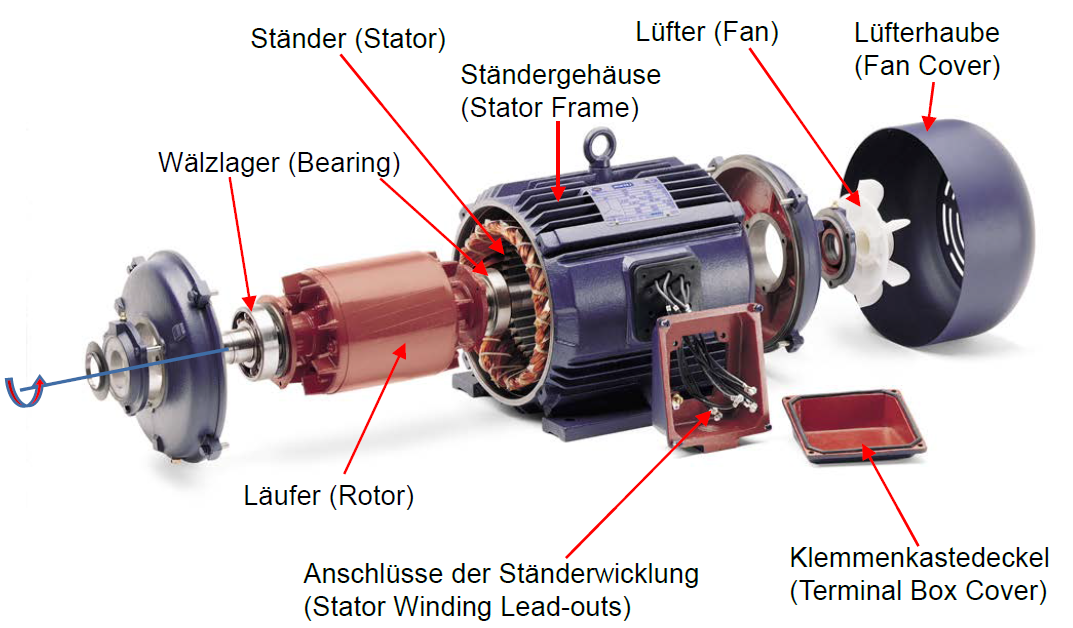
\includegraphics[scale = 0.3]{images/AsynchronmotorAufbau}
\end{minipage}
\begin{minipage}[b]{0.28\linewidth}
	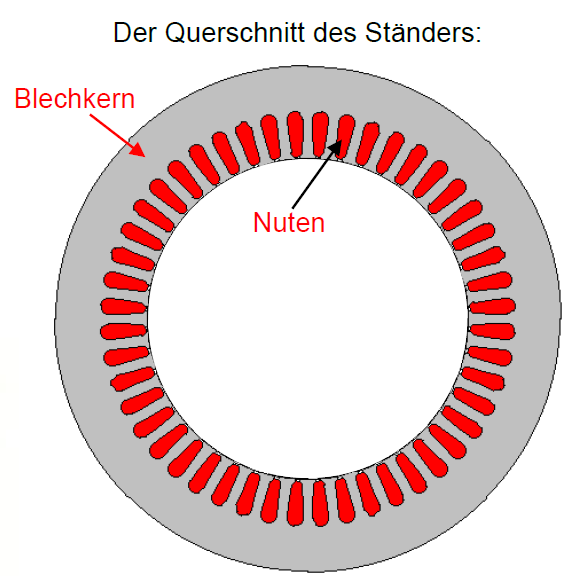
\includegraphics[scale = 0.3]{images/AQuerschnitt}
\end{minipage}
\begin{minipage}[b]{0.33\linewidth}
	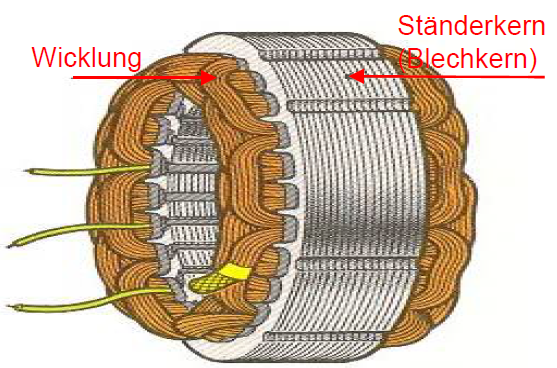
\includegraphics[scale = 0.4]{images/AsynchronmotorStaenderkern}
\end{minipage}\\
\subsection{Aufbau Läufer}
\begin{minipage}[b]{0.5\linewidth}
	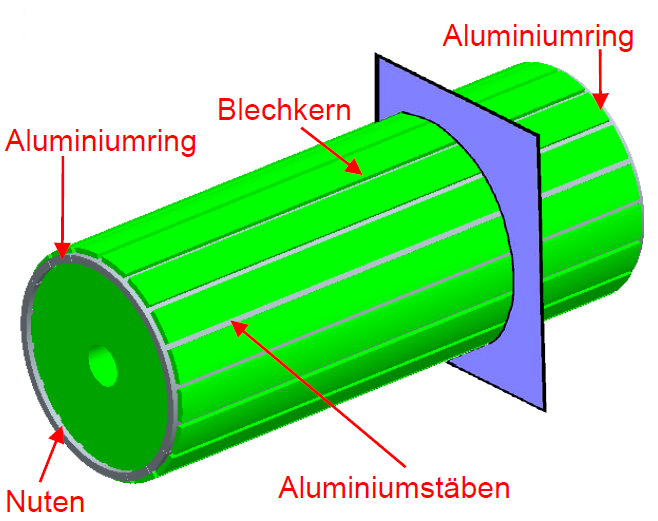
\includegraphics[scale = 0.4]{images/AsynchronRotor}
\end{minipage}
\begin{minipage}[b]{0.5\linewidth}
	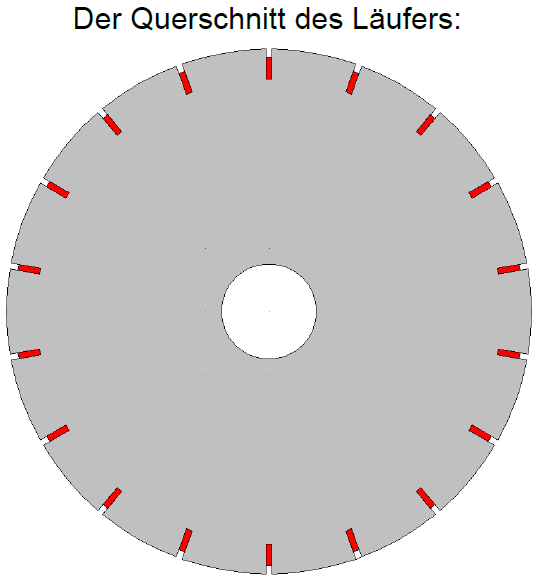
\includegraphics[scale = 0.4]{images/QuerschnittAsynchronrotor}
\end{minipage} \\\\
Wirbelströme im Eisen entstehen durch die Induktion des Rotors in den Stator \newline => Stator erwärmt sich.\newline Durch den Rillenaufbau des Stators können diese Wirbelströme bzw. die Temperaturansteigung minimiert \newline werden.\\


Schlupf $\widehat{=}$ der Abweichung zu der Synchronen Drehzahl 
\clearpage
\pagebreak
\subsection{Formeln Läufer}
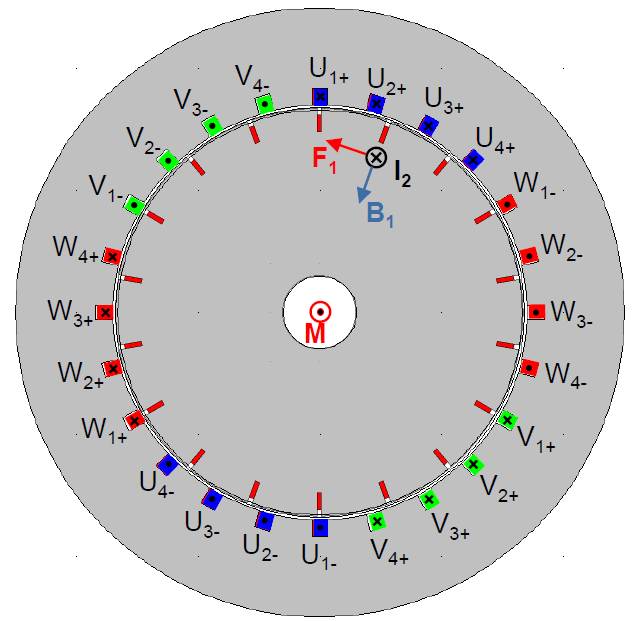
\includegraphics[scale = 0.5]{images/QuerschnittAmotor}\\\\
\begin{tabular}[b]{|C{4cm}| P{8cm} | P{5cm}|}
	\hline
	\textbf{Induzierte Spannung} & \begin{equation*}
	U_i = 4.44\cdot f\cdot w\cdot\xi\cdot\phi
	\end{equation*} & f $\widehat{=}$ Frequenz \newline w $\widehat{=}$ Windungszahl \newline $\xi$ = Wicklungsfaktor \newline $\phi$ = Magnetischer Fluss \\
	\hline
\textbf{Elektromagnetische Kraft}	& \begin{equation*} \vec{F_2} = I_2\cdot\vec{I_2}\times\vec{B_1}
\end{equation*} & \\
	\hline
\textbf{Mechanisches Drehmoment}	& \begin{equation*}
	\vec{M_2} = \vec{r_2}\times\vec{F_2}
\end{equation*} & \\
	\hline
	& & \\
	\hline
\end{tabular}
\clearpage
